\documentclass[14pt]{beamer}
\usetheme{Boadilla}
\usepackage{booktabs}
\usepackage{multirow}
\usepackage{enumitem}
\usepackage{tikz}

\newcommand{\E}{\mathbb{E}}
\usefonttheme{professionalfonts}
\usepackage{pgfplots}
\pgfplotsset{compat=1.18}
\renewcommand{\arraystretch}{1.25}
\usetikzlibrary{trees}
\title[ECON2843]{Lecture 15}
\subtitle{Part 3 Estimation and Hypothesis Test}
\date{}
\usepackage{amsmath,amssymb,mathtools,wasysym}
\begin{document}
	\begin{frame}
		\titlepage
	\end{frame}
	\begin{frame}
		\vspace{1cm}
		\centering
		{\color{blue}\large Continue our talk on hypothesis test}
	\end{frame}
	
\begin{frame}
	\frametitle{Importance of $p$-values}
	
	\begin{itemize}[label={\color{blue}$\blacktriangleright$}]
		\item How can we use $p$-values to conduct a hypothesis test?
		\item A very small $p$-value means that the observed test statistic was very extreme.
		\item So very small $p$-values should result in the rejection of $H_0$.
	\end{itemize}
	
\end{frame}
\begin{frame}
	\frametitle{Importance of $p$-values}
	
	\begin{itemize}[label={\color{blue}$\blacktriangleright$}]
		\item But how small is small?
		\item We can perform the hypothesis test by comparing the $p$-value to the significance level $\alpha$:
		\begin{itemize}[label={\color{blue}$\blacktriangleright$}]
			\item If the $p$-value is less than $\alpha$, we reject $H_0$.
			\item If the $p$-value is greater than $\alpha$, we fail to reject $H_0$.
		\end{itemize}
		\item Why?
		\item Suppose we test $H_0 : \mu = \mu_0$ vs $H_1 : \mu < \mu_0$ at $\alpha = 0.05$.
	\end{itemize}
	
\end{frame}

\begin{frame}
	\frametitle{Importance of $p$-values}
	
\centering
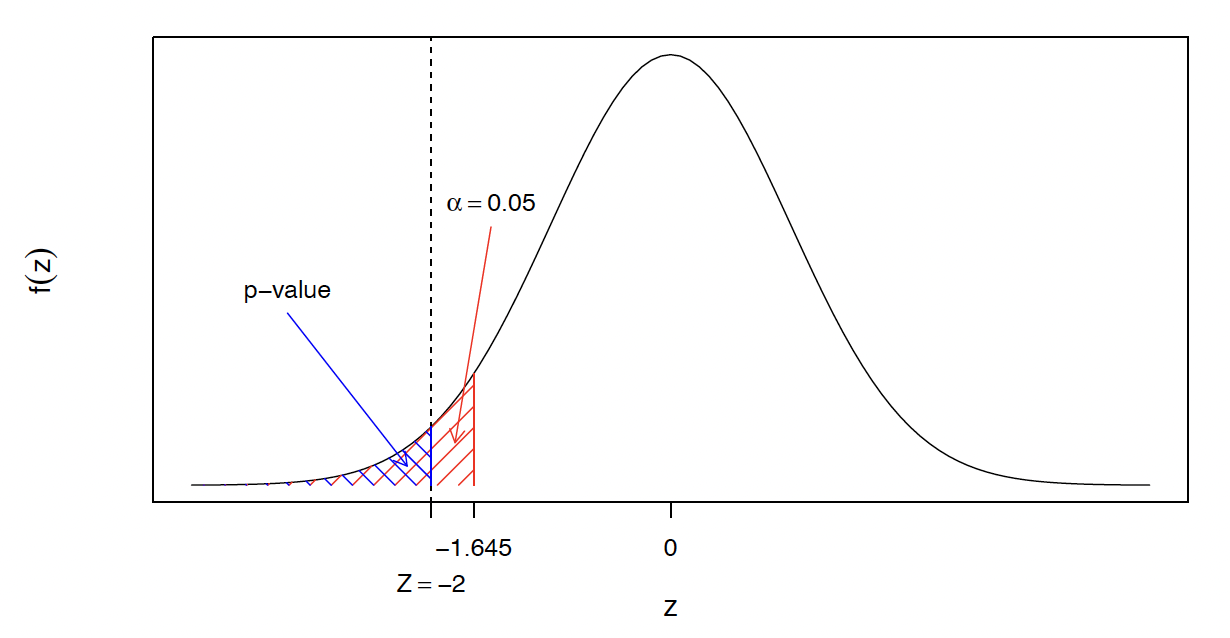
\includegraphics[width=11cm]{importance1.png}	
	
\end{frame}
\begin{frame}
	\frametitle{Importance of $p$-values}
	
	\centering
	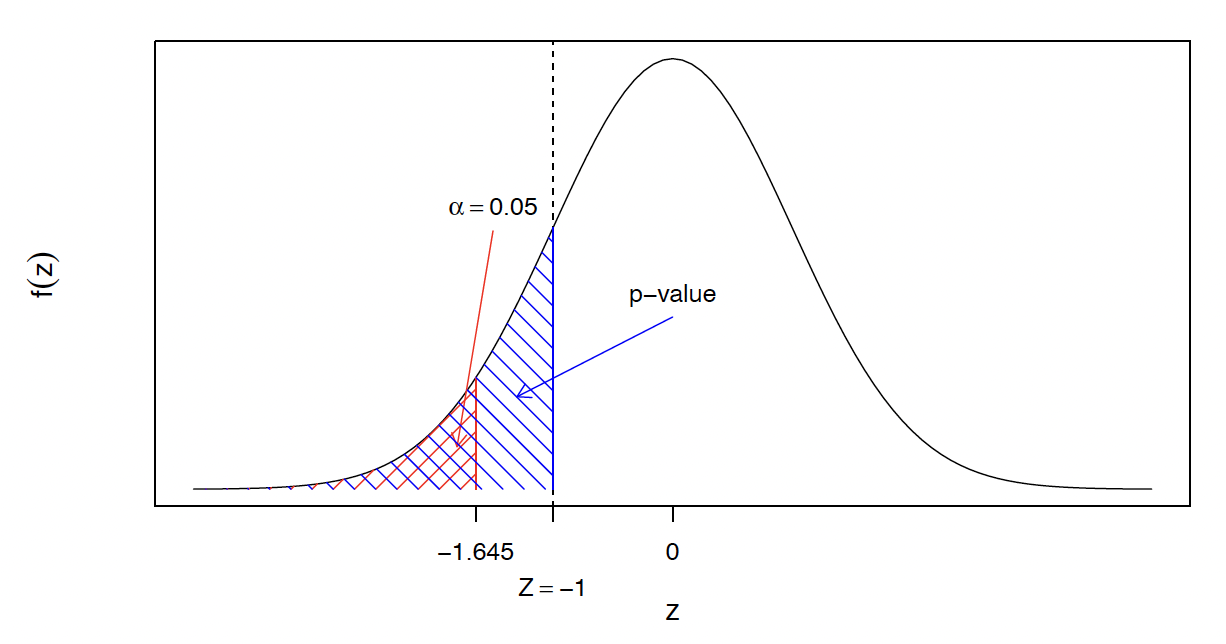
\includegraphics[width=11cm]{importance2.png}	
	
\end{frame}
\begin{frame}
	\frametitle{Importance of $p$-values}
	
	\begin{itemize}[label={\color{blue}$\blacktriangleright$}]
		\item Remember that rejection regions were calculated by finding the critical values that cut off $100\alpha\%$ in the extreme tail (one-tailed) or tails (two-tailed).
		
		\item If the $p$-value is less than $\alpha$, then the test statistic must lie within the rejection region, which means we reject $H_0$.
		
		\item If the $p$-value is greater than $\alpha$, then the test statistic must not lie within the rejection region, which means we fail to reject $H_0$.
	\end{itemize}
	
\end{frame}
\begin{frame}
	\frametitle{Another Bowling Example}
	
	\begin{itemize}[label={\color{blue}$\blacktriangleright$}]
		\item Your lecturer claims to have a bowling average of 150 or higher.
		
		\item You play 10 games with him, and he scores an average of 140.
		
		\item Suppose that the standard deviation for bowling scores is 15.
		
		\item Given a 5\% significance level, do you reject your lecturer's claim?
	\end{itemize}
	
\end{frame}

\begin{frame}
	\frametitle{Hypotheses and Test Statistic}
	
	\begin{enumerate}[label=\textcolor{blue}{\arabic*.}]
		\item State the hypotheses:
		\[
		\begin{aligned}
			H_0 : \mu &= 150 \\
			H_1 : \mu &< 150
		\end{aligned}
		\]
		
		\item Standardize $\bar{X}$ to get the test statistic:
		\[
		Z = \frac{140 - 150}{\frac{15}{\sqrt{10}}} = -2.1082
		\]
	\end{enumerate}
	
\end{frame}
\begin{frame}
	\frametitle{Decision Rule and Conclusion}
	
	\begin{enumerate}[label=\textcolor{blue}{\arabic*.}]
		\item The $p$-value is: $P(Z<-2.1082)=0.0174$.
		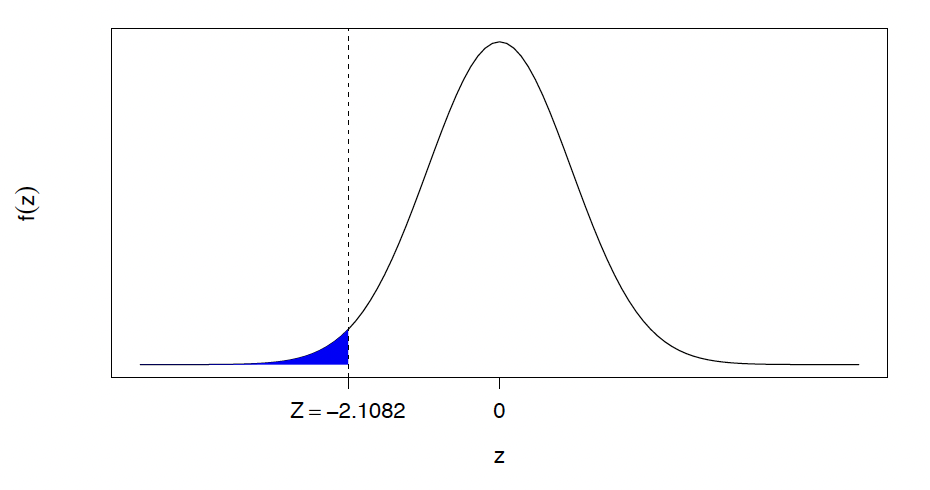
\includegraphics[width=8cm]{desision.png}
		\item Since $p$-value $<\alpha$, i.e., $0.0174<0.05$, we reject $H_0$ and conclude my bowling average is less than $150$.
	\end{enumerate}
	
\end{frame}
\begin{frame}
	\frametitle{Decision Rule and Conclusion}
\centering
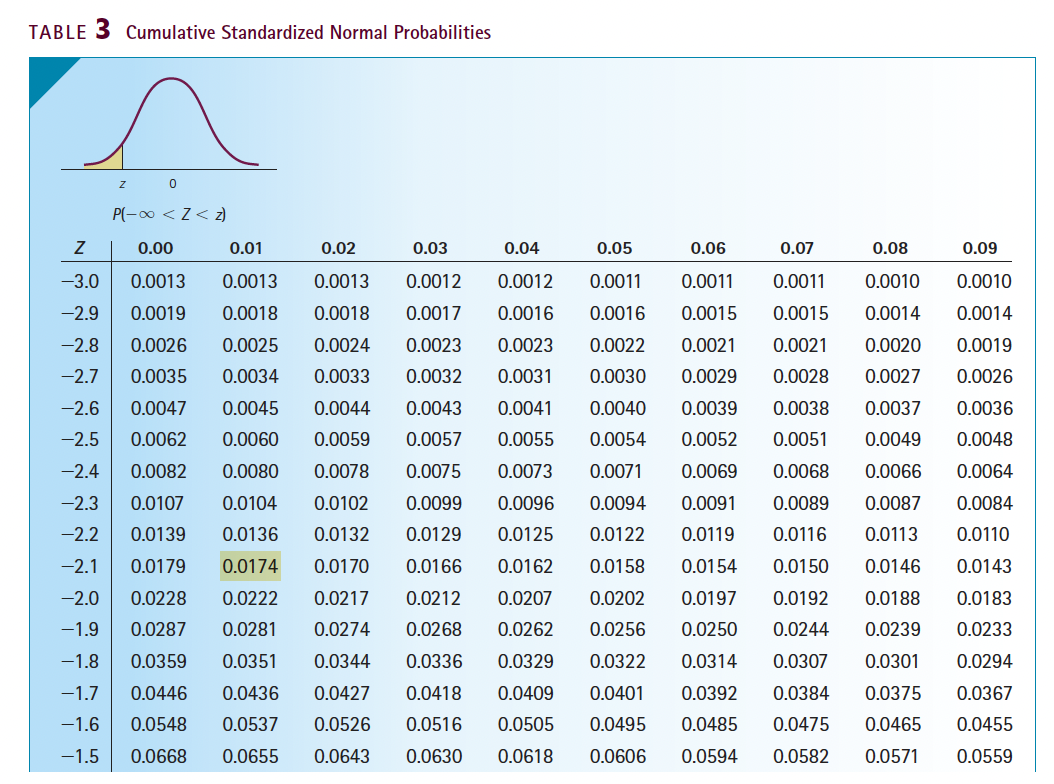
\includegraphics[width=10cm]{ztable.png}	
\end{frame}
\begin{frame}
	\frametitle{Using $p$-values}
	
	\begin{itemize}[label={\color{blue}$\blacktriangleright$}]
		\item The conclusions we draw from using the rejection region method and the $p$-value method are always \emph{exactly} the same.
		
		\item When calculating $p$-values for two-tailed tests, remember that ``more extreme'' includes the situations when the test statistic is too small \emph{or} too big. We care about \emph{both} tails.
		
		\item Using $p$-values is a more elegant and flexible way of performing hypothesis tests than using rejection regions.
	\end{itemize}
	
\end{frame}
\begin{frame}
	\frametitle{Confidence Intervals}
	
	\begin{itemize}[label={\color{blue}$\blacktriangleright$}]
		\item Confidence intervals for $\mu$ and standardized test statistics used in hypothesis tests for $\mu$ are both derived from the sampling distribution of $\bar{X}$.
		
		\item Let's take a brief moment to compare a $100(1-\alpha)\%$ confidence interval and a two-tailed hypothesis test at a significance level of $\alpha$.
	\end{itemize}
	
\end{frame}

\begin{frame}
	\frametitle{Hypothesis Tests and Confidence Intervals}
	
	\begin{itemize}[label={\color{blue}$\blacktriangleright$}]
		\item Confidence interval is given by:
		\[
		\left(\bar{X} - z_{\frac{\alpha}{2}}\frac{\sigma}{\sqrt{n}}, \bar{X} + z_{\frac{\alpha}{2}}\frac{\sigma}{\sqrt{n}}\right)
		\]
		
		\item We reject a two-tailed hypothesis test at a significance level of $\alpha$ if:
		\[
		\frac{\bar{X} - \mu_0}{\frac{\sigma}{\sqrt{n}}} < -z_{\frac{\alpha}{2}} \quad \text{or} \quad \frac{\bar{X} - \mu_0}{\frac{\sigma}{\sqrt{n}}} > z_{\frac{\alpha}{2}}
		\]
	\end{itemize}
	
\end{frame}
\begin{frame}
	\frametitle{Hypothesis Tests and Confidence Intervals}
	
	\begin{itemize}[label={\color{blue}$\blacktriangleright$}]
		\item Starting with the lower rejection region and rearranging, we get:
		\[
		\begin{aligned}
			&\frac{\bar{X} - \mu_0}{\frac{\sigma}{\sqrt{n}}} < -z_{\frac{\alpha}{2}} \\[1ex]
			\Rightarrow \quad &\bar{X} - \mu_0 < -z_{\frac{\alpha}{2}}\frac{\sigma}{\sqrt{n}} \\[1ex]
			\Rightarrow \quad &\mu_0 > \bar{X} + z_{\frac{\alpha}{2}}\frac{\sigma}{\sqrt{n}}
		\end{aligned}
		\]
		
		\item We can perform a similar rearrangement for the upper rejection region.
	\end{itemize}
	
\end{frame}

\begin{frame}
	\frametitle{Hypothesis Tests and Confidence Intervals}
	
	\begin{itemize}[label={\color{blue}$\blacktriangleright$}]
		\item Inspecting these carefully, it becomes clear that constructing a confidence interval is equivalent to performing a \emph{two-tailed} hypothesis test.
		
		\item If the value of $\mu_0$ in the null hypothesis falls \emph{outside} the calculated confidence interval, we \emph{reject} the null hypothesis.
		
		\item If it falls \emph{inside} the calculated confidence interval, we \emph{do not reject} the null hypothesis.
	\end{itemize}
	
\end{frame}
\begin{frame}
	\frametitle{Type I and Type II Errors}
	
	\begin{itemize}[label={\color{blue}$\blacktriangleright$}]
		\item Type I error occurs when we reject the null hypothesis when it is true.
		\begin{itemize}[label={\color{blue}$\blacktriangleright$}]
			\item $P(\text{Type I error}) = \alpha$, the significance level of the test.
		\end{itemize}
		
		\item Type II error occurs when we fail to reject the null hypothesis when it is not true.
		\begin{itemize}[label={\color{blue}$\blacktriangleright$}]
			\item $P(\text{Type II error}) = \beta$.
			\item The \textbf{power} of a test is defined to be $1 - \beta$.
		\end{itemize}
	\end{itemize}
	
\end{frame}
\begin{frame}
	\frametitle{Probability of a Type II Error}
	
	\begin{itemize}[label={\color{blue}$\blacktriangleright$}]
		\item Calculating $P(\text{Type II error})$ involves finding the probability of not rejecting $H_0$ (i.e., the test statistic not falling in the rejection region) when $H_1$ is true (i.e., under the ``alternative distribution'').
		
		\item To do this we need to know:
		\begin{itemize}[label={\color{blue}$\blacktriangleright$}]
			\item The rejection region.
			\item The true value of the parameter under $H_1$.
		\end{itemize}
	\end{itemize}
	
\end{frame}
\begin{frame}
	\frametitle{Probability of a Type II Error}
	
	\begin{itemize}[label={\color{blue}$\blacktriangleright$}]
		\item $P(\text{Type II error})$ can generally be calculated using the following steps:
	\end{itemize}
	
	\begin{enumerate}[label=\textcolor{blue}{\arabic*.}]
		\item Based on $\alpha$ and the hypotheses, determine the rejection region in terms of the standardized test statistic.
		
		\item Works backwards to determine the rejection region in terms of the \emph{unstandardized} test statistic.
		
		\item Calculate the probability of not rejecting $H_0$, under $H_1$, by re-standardizing using the true value of the parameter.
	\end{enumerate}
	
\end{frame}
\begin{frame}
	\frametitle{Example}
	
	\begin{itemize}[label={\color{blue}$\blacktriangleright$}]
		\item You want to test the claim that the average house price in your suburb is not below \$400,000. The average of the most recent five sales is equal to \$420,000. The standard deviation of house prices is \$20,000.
		
		\item Given that the true average house price is in fact \$390,000, calculate the probability of a type II error and the power of the test, at a 5 percent significance level.
	\end{itemize}
	
\end{frame}
\begin{frame}
	\frametitle{Hypotheses}
	
	\begin{itemize}[label={\color{blue}$\blacktriangleright$}]
		\item Note that the claim given in the question is $\mu \geq 400\,000$. So the hypotheses are:
		
		\[
		\begin{aligned}
			H_0 : \mu &= 400\,000 \\
			H_1 : \mu &< 400\,000
		\end{aligned}
		\]
		
		\item This is a one-tailed (lower-tailed) test.
	\end{itemize}
	
\end{frame}
\begin{frame}
	\frametitle{Null Distribution and Rejection Region}
	
	\centering
	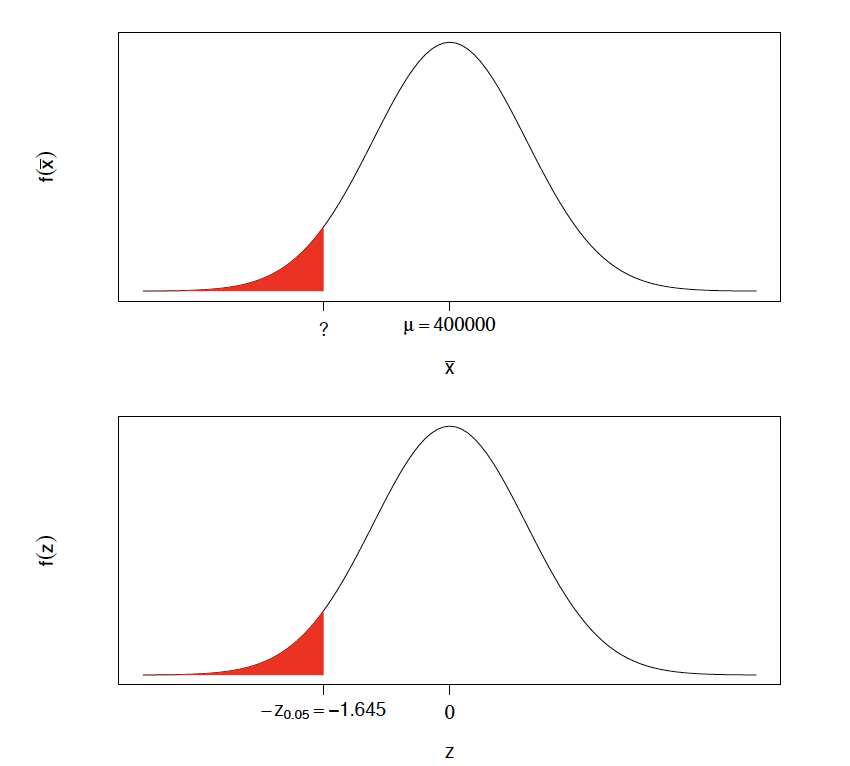
\includegraphics[width=9cm]{null.png}	
	
\end{frame}
\begin{frame}
	\frametitle{Null Distribution and Rejection Region}
	
	\begin{itemize}[label={\color{blue}$\blacktriangleright$}]
		\item We need to convert the rejection region in terms of the standardized $Z$-statistic, i.e., $Z < -1.645$, into a rejection region in terms of the unstandardized $\bar{X}$:
	\end{itemize}
	
	\begin{align*}
		Z &< -1.645 \\[1ex]
		\Rightarrow \frac{\bar{X} - \mu_0}{\frac{\sigma}{\sqrt{n}}} &< -1.645 \\[1ex]
		\Rightarrow \frac{\bar{X} - 400\,000}{\frac{20\,000}{\sqrt{5}}} &< -1.645 \\[1ex]
		\Rightarrow \bar{X} &< 385\,286.7
	\end{align*}
	
\end{frame}
\begin{frame}
	\frametitle{Null Distribution and Rejection Region}
	\centering
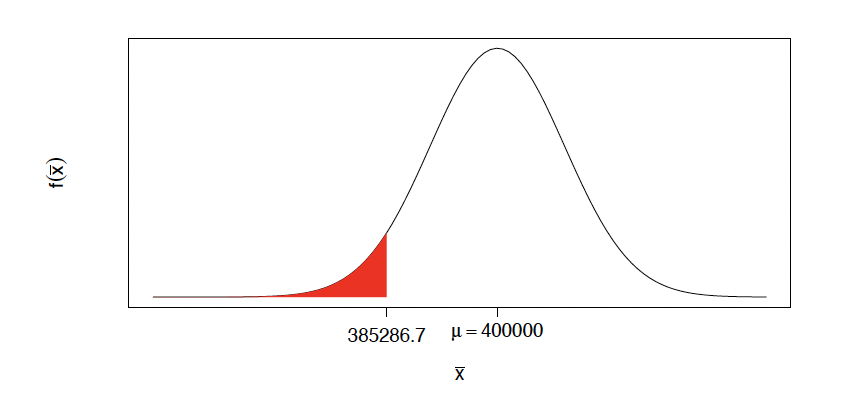
\includegraphics[width=9cm]{null2.png}	
\end{frame}
\begin{frame}
	\frametitle{Probability of a Type II Error}
	\centering
	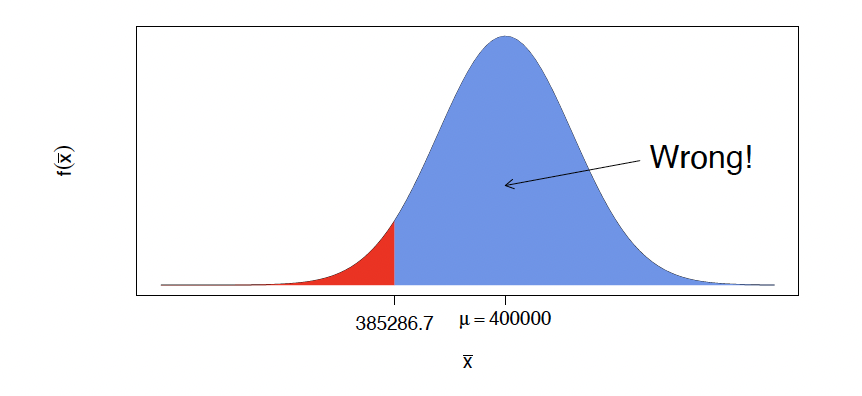
\includegraphics[width=9cm]{type2.png}	
\end{frame}
\begin{frame}
	\frametitle{Probability of a Type II Error}
	\centering
	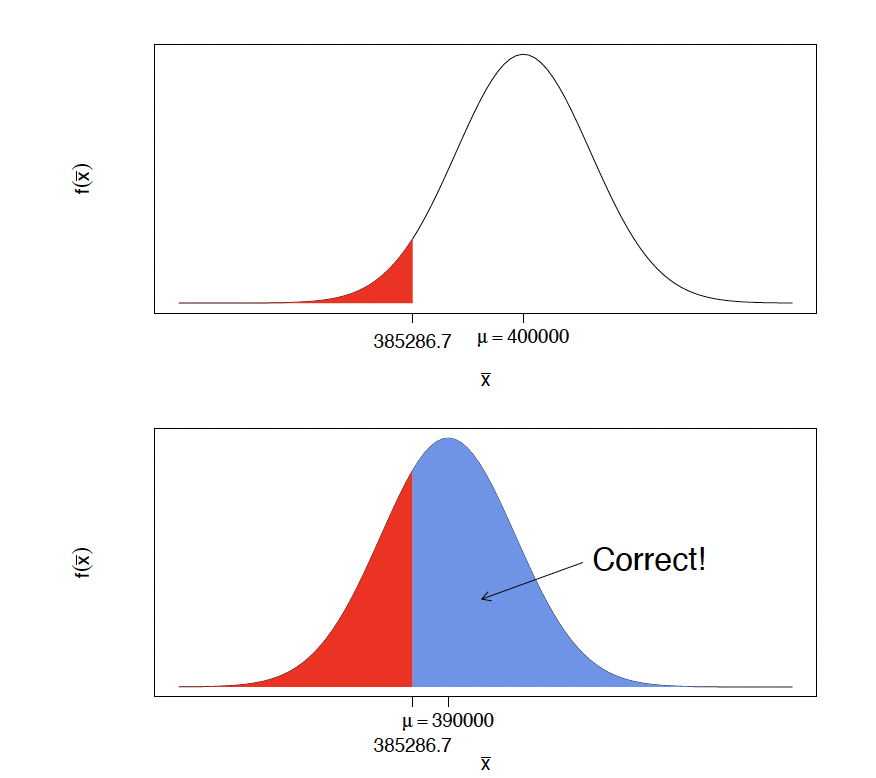
\includegraphics[width=9cm]{type22.png}	
\end{frame}
\begin{frame}
	\frametitle{Probability of a Type II Error}
	
	\begin{itemize}[label={\color{blue}$\blacktriangleright$}]
		\item To calculate $P(\text{Type II error})$ we need to standardize with respect to the true value of $\mu$ under $H_1$, i.e., $\mu = 390\,000$:
	\end{itemize}
	
	\begin{align*}
		P(\text{Type II error}) &= P(\bar{X} > 385\,286.7 \mid H_1 \text{ is true}) \\[1ex]
		&= P\left(\frac{\bar{X} - \mu}{\frac{\sigma}{\sqrt{n}}} > \frac{385\,286.7 - \color{red}390\,000\color{black}}{\frac{20\,000}{\sqrt{5}}}\right) \\[1ex]
		&= P(Z > -0.5270) \\[1ex]
		&= 1 - P(Z < -0.5270) \\[1ex]
		&= 0.7019
	\end{align*}
	
\end{frame}
\begin{frame}
	\frametitle{Probability of a Type II Error}
	
	\begin{itemize}[label={\color{blue}$\blacktriangleright$}]
		\item So if the true average house price is actually \$390\,000, then the probability of making a type II error is $\beta = 0.7019$, which is relatively high.
		
		\item This means the power of the test is equal to $1 - \beta = 0.2981$.
		
		\item Note that the $\beta = P(\text{Type II error})$ depends on both $\alpha$ and the true value of $\mu$ under $H_1$.
	\end{itemize}
	
\end{frame}
	\begin{frame}
	\vspace{1cm}
	\centering
	{\color{blue}\large Hypothesis Test for $\mu$ when $\sigma^2$ is Unknown}
\end{frame}

\begin{frame}
	\frametitle{Hypothesis Test for $\mu$ when $\sigma^2$ is Unknown}
	
	\begin{itemize}[label={\color{blue}$\blacktriangleright$}]
		\item When we know $\sigma^2$, hypothesis tests for $\mu$ use the standardized $Z$-statistic as the test statistic:
		
		\[
		Z = \frac{\bar{X} - \mu_0}{\frac{\sigma}{\sqrt{n}}}
		\]
		
		\item The null distribution of $Z$ was $N(0,1)$ (for large $n$), so we can determine rejection regions and calculate $p$-values by looking up the $z$-tables.
		
		\item What happens if we don't know $\sigma^2$?
	\end{itemize}
	
\end{frame}

\begin{frame}
	\frametitle{We Often Don't Know the Population Variance $\sigma^2$}
	\begin{itemize}[label={\color{blue}$\blacktriangleright$}]
		\item In many real-world scenarios, the population variance is unknown
		\item Examples:
		\begin{itemize}[label={\color{blue}$\blacktriangleright$}]
			\item Variance of height of all the OU students.
			\item Medical research: Testing a new drug's effectiveness
			\item Quality control: Assessing product consistency in manufacturing
			\item Social sciences: Studying income distribution in a large population
		\end{itemize}
	\end{itemize}
\end{frame}

\begin{frame}
	\frametitle{Hypothesis Test for $\mu$ when $\sigma^2$ is Unknown}
	
	\begin{itemize}[label={\color{blue}$\blacktriangleright$}]
		\item {\color{red}We can estimate $\sigma^2$ using the sample variance $s^2$.}
		\item So let's replace $\sigma$ in the $Z$-statistic with $s$:
		\[
		T = \frac{\bar{X} - \mu_0}{\frac{s}{\sqrt{n}}}
		\]
		\item {\color{blue}Under $H_0$, this ``$T$-statistic'' no longer has a $N(0,1)$ distribution, so we can't perform the test by looking up the $z$-tables.}
		\item But if we knew the null distribution of $T$, we could still perform the test...
	\end{itemize}
	
\end{frame}
\begin{frame}
	\frametitle{$t$-distribution}
	
	\begin{itemize}[label={\color{blue}$\blacktriangleright$}]
		\item The null distribution of this $T$-statistic is the $t$-distribution with $n - 1$ degrees of freedom.
		\item The $t$-distribution is a special continuous distribution:
		\begin{itemize}[label={\color{blue}$\blacktriangleright$}]
			\item It's symmetric about 0 and bell shaped, just like the standard normal distribution.
			\item It has one parameter called the degrees of freedom, and as this increases, the $t$-distribution approaches the standard normal distribution.
			\item It has a greater variance than the standard normal distribution.
		\end{itemize}
	\end{itemize}
	
\end{frame}
\begin{frame}
	\frametitle{$t$-distribution}
	\centering
	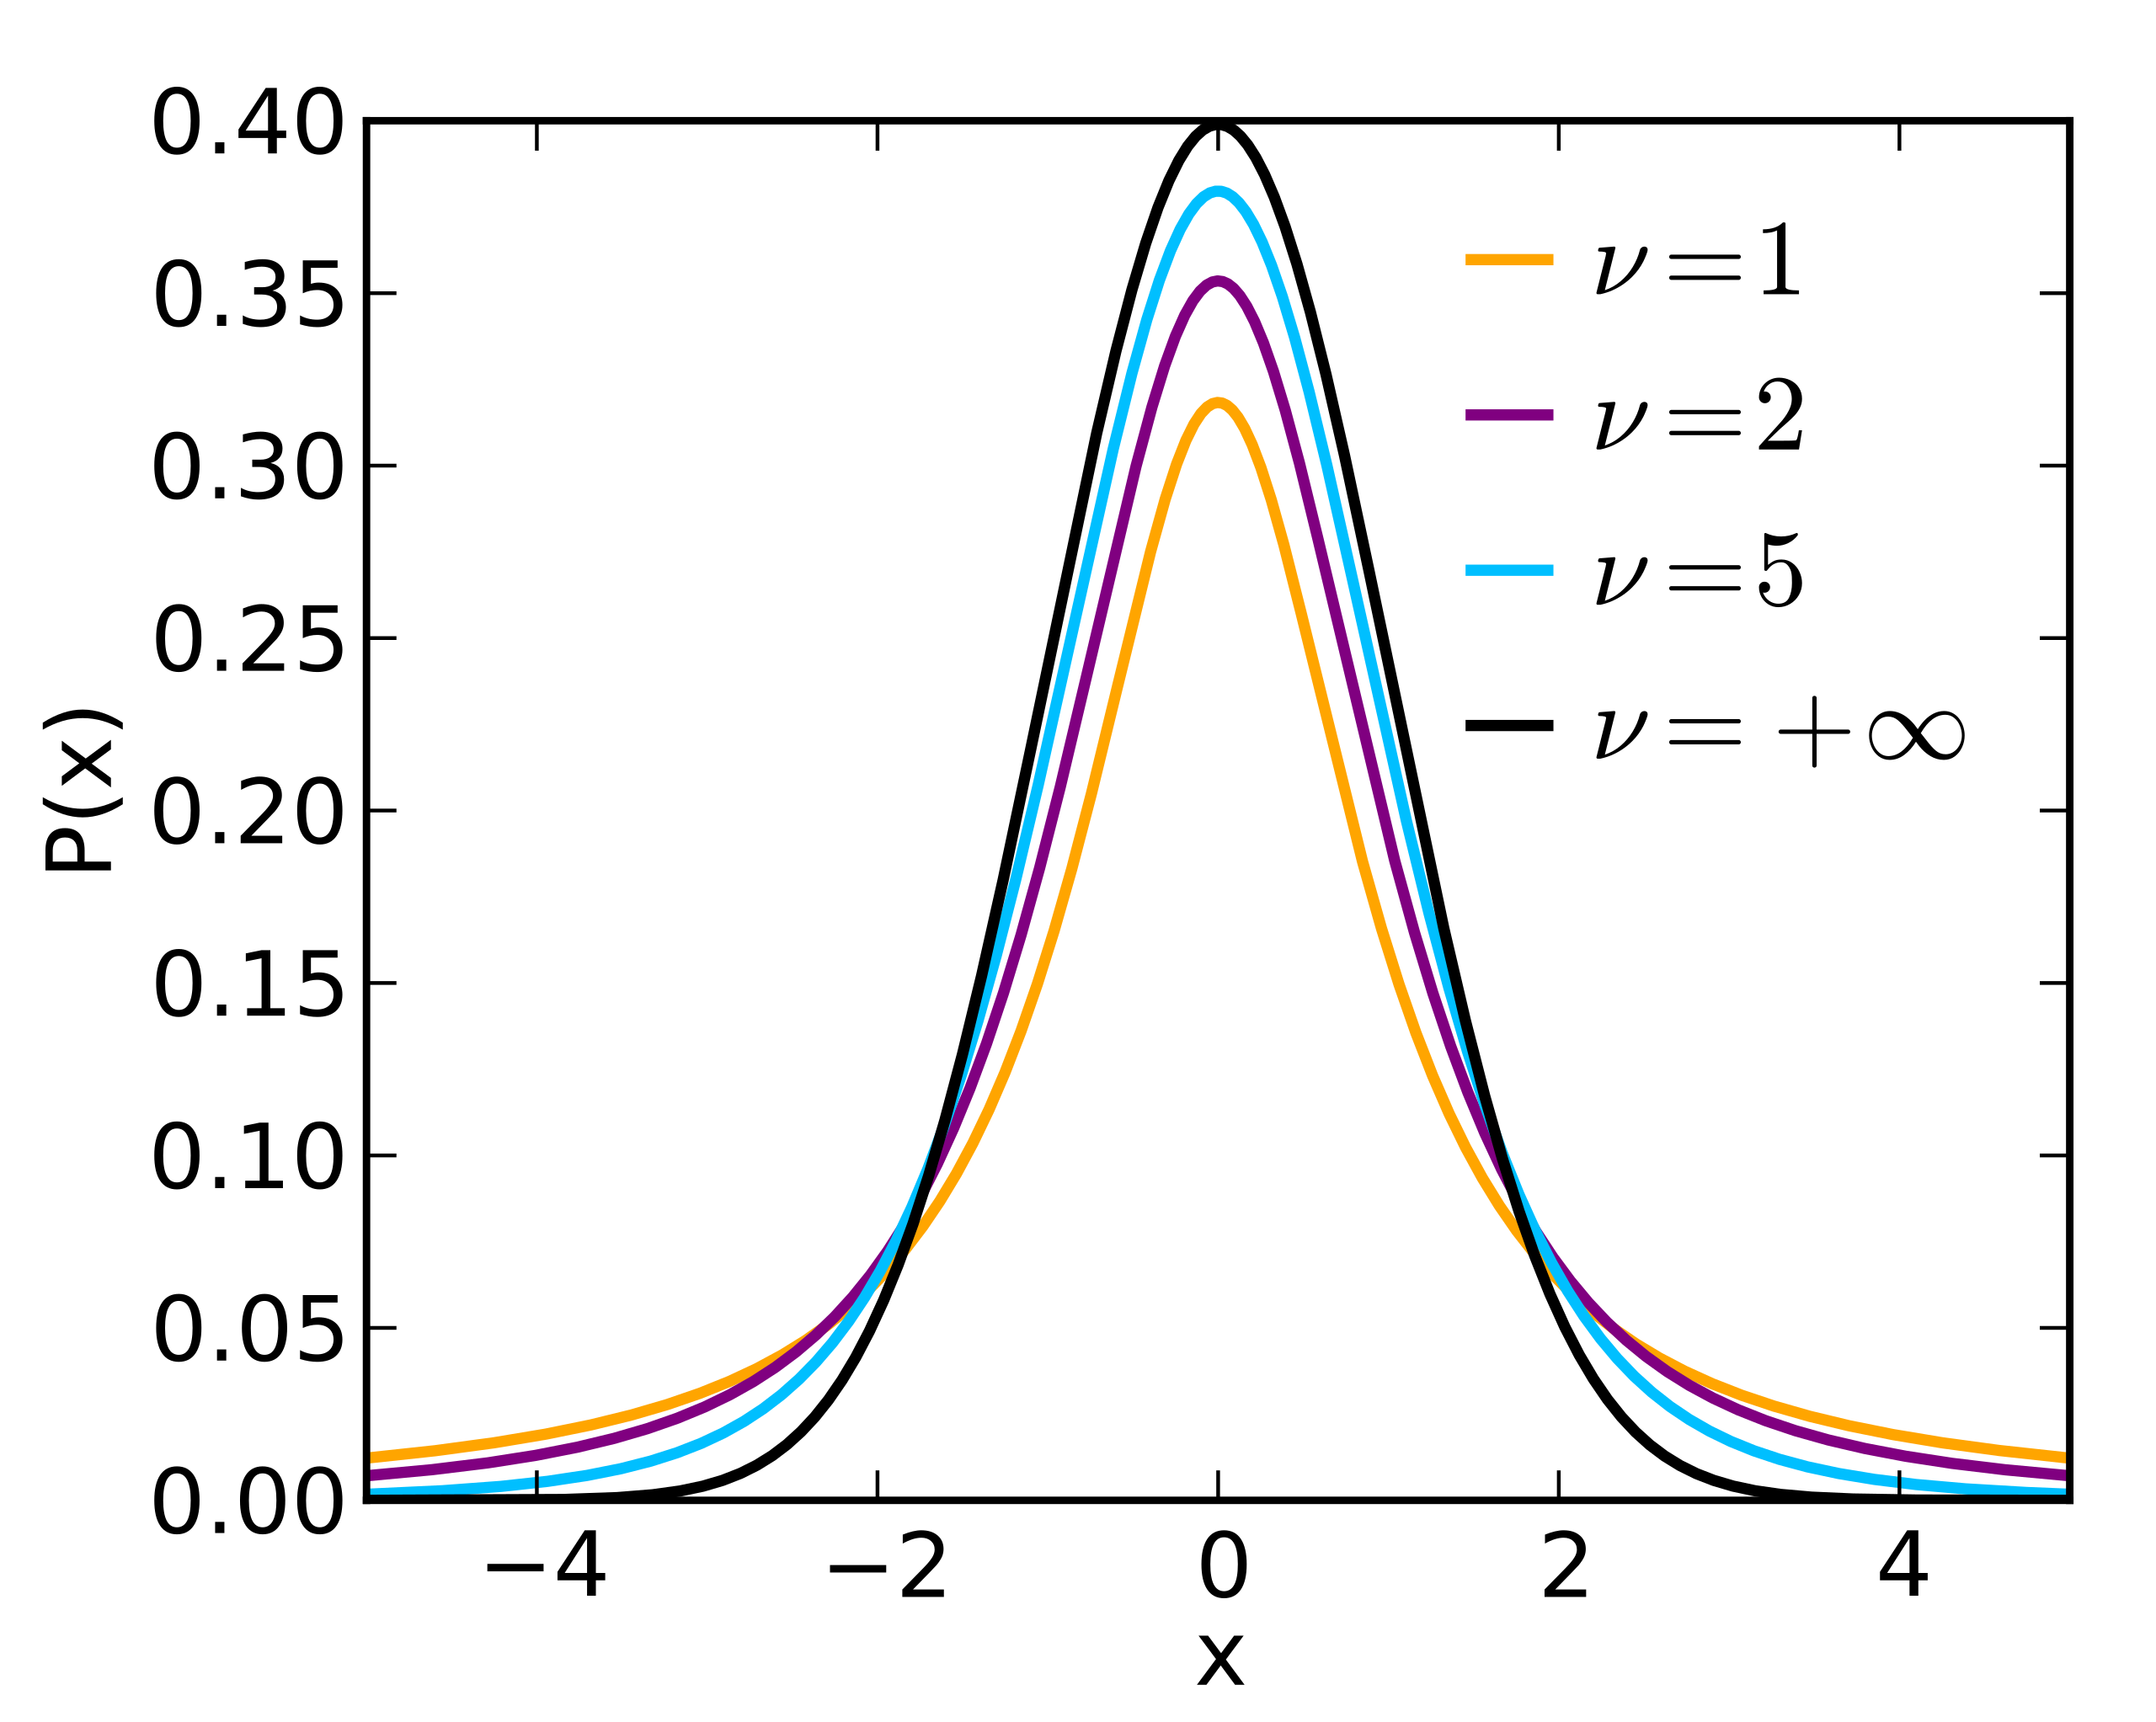
\includegraphics[width=9cm]{t.png}	
\end{frame}
\begin{frame}
	\frametitle{Let's use the Bowling Example}
	
	\begin{itemize}[label={\color{blue}$\blacktriangleright$}]
		\item Your lecturer claims to have a bowling average of 150 or higher.
		
		\item You play 10 games with him, and he scores an average of 140.
		
		\item The population standard deviation of bowling scores is unknown. However, for these 10 games, you calculate the sample standard deviation to be 13.7.
		
		\item Given a 5\% significance level, do you reject your lecturer's claim?
	\end{itemize}
	
\end{frame}
\begin{frame}
	\frametitle{Hypotheses and Test Statistic}
	
	\begin{itemize}[label={\color{blue}$\blacktriangleright$}]
		\item Hypotheses:
		\[
		\begin{aligned}
			H_0 : \mu &= 150 \\
			H_1 : \mu &< 150
		\end{aligned}
		\]
		
		\item Test statistic:
		\[
		T = \frac{\bar{X} - \mu_0}{\frac{s}{\sqrt{n}}} = \frac{140 - 150}{\frac{13.7}{\sqrt{10}}} = -2.3082
		\]
	\end{itemize}
	
\end{frame}
\begin{frame}
	\frametitle{Null Distribution}
	\centering
	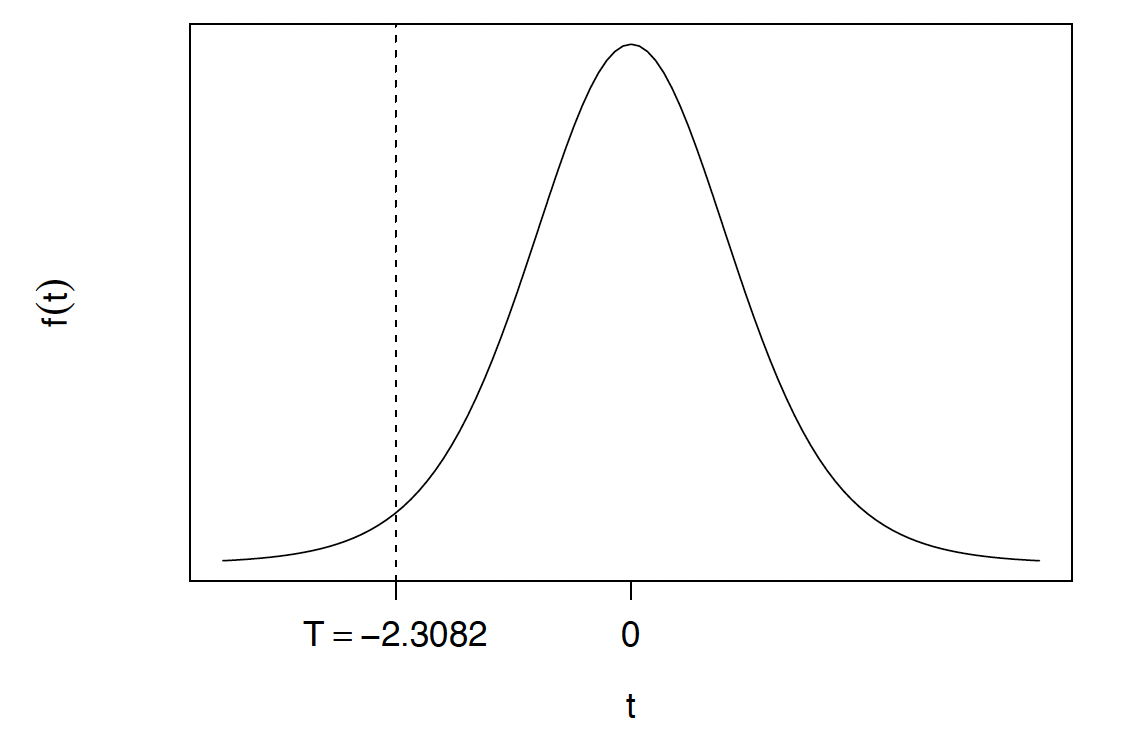
\includegraphics[width=10cm]{nullt.png}	
\end{frame}
\begin{frame}
	\frametitle{Decision Rule}
	
	\begin{itemize}[label={\color{blue}$\blacktriangleright$}]
		\item We need to determine the rejection region.
		
		\item That is, we must find the critical value that cuts off 5\% in the lower tail of a $t$-distribution with $n - 1 = 9$ degrees of freedom.
		
		\item From the symmetry of the $t$-distribution about 0, the rejection region is given by $T < -1.833$.
	\end{itemize}
	
\end{frame}
\begin{frame}
	\frametitle{Decision Rule}
	\centering
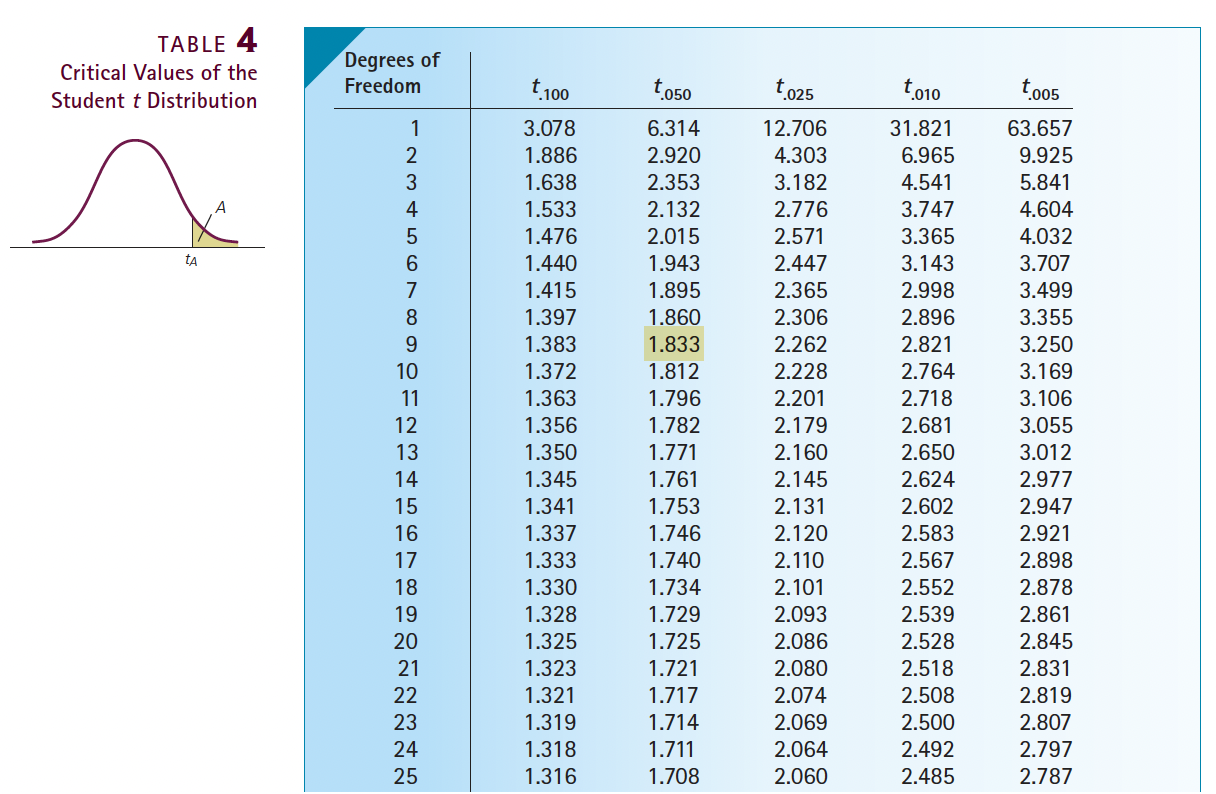
\includegraphics[width=10cm]{decision.png}	
\end{frame}
\begin{frame}
	\frametitle{Conclusion}
\begin{itemize}[label={\color{blue}$\blacktriangleright$}]
	\item Since $-2.3082<-1.833$, we reject $H_0$ and conclude that my bowling average is less than 150.
\end{itemize}
	\centering
	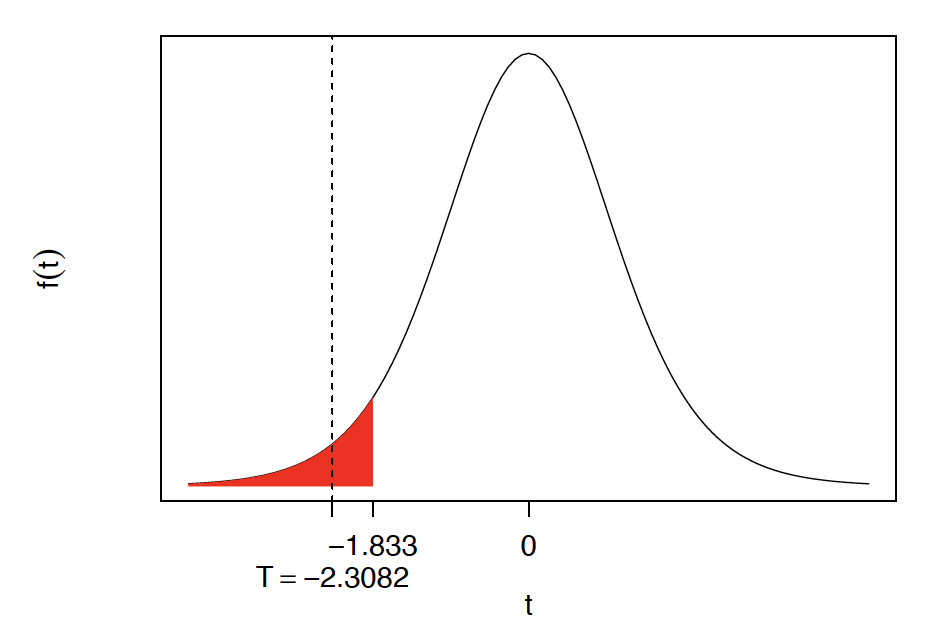
\includegraphics[width=10cm]{conclusion.png}	
\end{frame}
\begin{frame}
	\frametitle{Confidence Interval}
	
	\begin{itemize}[label={\color{blue}$\blacktriangleright$}]
		\item We know that calculating a confidence interval is the same as performing a two-tailed hypothesis test.
		
		\item A $100(1-\alpha)\%$ confidence interval for $\mu$ when $\sigma^2$ is unknown is given by:
		
		\[
		\left(\bar{X} - t_{\frac{\alpha}{2},n-1}\frac{s}{\sqrt{n}}, \bar{X} + t_{\frac{\alpha}{2},n-1}\frac{s}{\sqrt{n}}\right)
		\]
		
		\item NB: $t_{\frac{\alpha}{2},n-1}$ is the value that cuts off an area of $\frac{\alpha}{2}$ in the upper tail of the $t$-distribution with $n-1$ degrees of freedom.
	\end{itemize}
	
\end{frame}
	\begin{frame}
	\vspace{1cm}
	\centering
	{\color{blue}\large Hypothesis Test for Sample Proportion $p$}
\end{frame}
\begin{frame}
	\frametitle{Hypothesis Test for $p$}
	
	\begin{itemize}[label={\color{blue}$\blacktriangleright$}]
		\item Suppose we are now interested in making inferences about a population proportion $p$.
		\begin{itemize}[label={\color{blue}$\blacktriangleright$}]
			\item For example, the population proportion of people who prefer Coke over Pepsi.
		\end{itemize}
		
		\item How would we test the following hypotheses?
		
		\[
		\begin{aligned}
			H_0 : p &= p_0 \\
			H_1 : p(&\neq, <, >)p_0
		\end{aligned}
		\]
	\end{itemize}
	
\end{frame}
\begin{frame}
	\frametitle{Hypothesis Test for $p$}
	
	\begin{itemize}[label={\color{blue}$\blacktriangleright$}]
		\item We can estimate a population proportion by the sample proportion:
		\[
		\hat{p} = \frac{X}{n}
		\]
		where $X$ is the number of successes in the sample and $n$ is the sample size.
		
		\item From previous topics we know that, for large $n$, the sampling distribution of $\hat{p}$ is:
		\[
		\hat{p} \sim N\left(p, \frac{p(1-p)}{n}\right)
		\]
	\end{itemize}
	
\end{frame}
\begin{frame}
	\frametitle{Hypothesis Test for $p$}
	
	\begin{itemize}[label={\color{blue}$\blacktriangleright$}]
		\item To perform hypothesis tests for $p$, we can then use the $Z$-statistic obtained by standardizing $\hat{p}$:
		
		\[
		Z = \frac{\hat{p} - p_0}{\sqrt{\frac{p_0(1-p_0)}{n}}}
		\]
		
		\item Since $Z \sim N(0,1)$ under $H_0$, we can then proceed as we normally do using the $z$-tables.
	\end{itemize}
	
\end{frame}
\begin{frame}
	\frametitle{Confidence Interval}
	
	\begin{itemize}[label={\color{blue}$\blacktriangleright$}]
		\item A $100(1-\alpha)\%$ confidence interval for a population proportion $p$ is given by:
		
		\[
		\left(\hat{p} - z_{\frac{\alpha}{2}} \sqrt{\frac{\hat{p}(1-\hat{p})}{n}}, \hat{p} + z_{\frac{\alpha}{2}} \sqrt{\frac{\hat{p}(1-\hat{p})}{n}}\right)
		\]
		
		\item Note that inside the square root we replaced $p_0$ with $\hat{p}$, since in an estimation setting we don't know the true value of $p$ and there is no hypothesized value $p_0$.
	\end{itemize}
	
\end{frame}
\begin{frame}
	\frametitle{Example}
	
	\begin{itemize}[label={\color{blue}$\blacktriangleright$}]
		\item The number of operators at a call center depends on the level of use.
		
		\item At random times over a brief interval, the call center is checked to see whether all operators are busy so as to assess the proportion of time all operators are busy.
		
		\item An additional operator will be employed if there is sufficient evidence that all operators are busy more than 80\% of the time.
	\end{itemize}
	
\end{frame}
\begin{frame}
	\frametitle{Example}
	
	\begin{itemize}[label={\color{blue}$\blacktriangleright$}]
		\item Twenty-five random times are chosen for checking and it was found that all operators were busy 96\% of the time.
		
		\item Would you recommend employing an additional operator in the call center?
		
		\item Population parameter of interest is $p$, the proportion of time that all operators are busy.
		
		\item We know that $n = 25$ and $\hat{p} = 0.96$.
	\end{itemize}
	
\end{frame}
\begin{frame}
	\frametitle{Hypotheses and Test Statistic}
	
	\begin{itemize}[label={\color{blue}$\blacktriangleright$}]
		\item Hypotheses:
		\[
		\begin{aligned}
			H_0 : p &= 0.8 \\
			H_1 : p &> 0.8
		\end{aligned}
		\]
		
		\item Test statistic (assume $H_0$ is true):
		\[
		Z = \frac{\hat{p} - p_0}{\sqrt{\frac{p_0(1-p_0)}{n}}} = \frac{0.96 - 0.8}{\sqrt{\frac{0.8(1-0.8)}{25}}} = 2
		\]
	\end{itemize}
	
\end{frame}
\begin{frame}
	\frametitle{Decision Rule and Conclusion}
	
	\begin{itemize}[label={\color{blue}$\blacktriangleright$}]
		\item Decision rule:
		\begin{itemize}[label={\color{blue}$\blacktriangleright$}]
			\item Calculate the $p$-value from the $z$-tables:
			\[
			p\text{-value} = P(Z > 2) = 0.0228
			\]
		\end{itemize}
		
		\item Conclusion:
		\begin{itemize}[label={\color{blue}$\blacktriangleright$}]
			\item Since $0.0228 < 0.05$, we reject $H_0$ at the 5\% significance level.
			\item We would conclude there is strong evidence that the proportion of time all operators are busy is greater than 80\% and recommend that a new operator be employed.
		\end{itemize}
	\end{itemize}
	
\end{frame}
\end{document}